\documentclass[11pt]{article}
\usepackage{amsthm,amssymb,amsmath}
\usepackage{color}
\usepackage{pgf,tikz}

\begin{document}

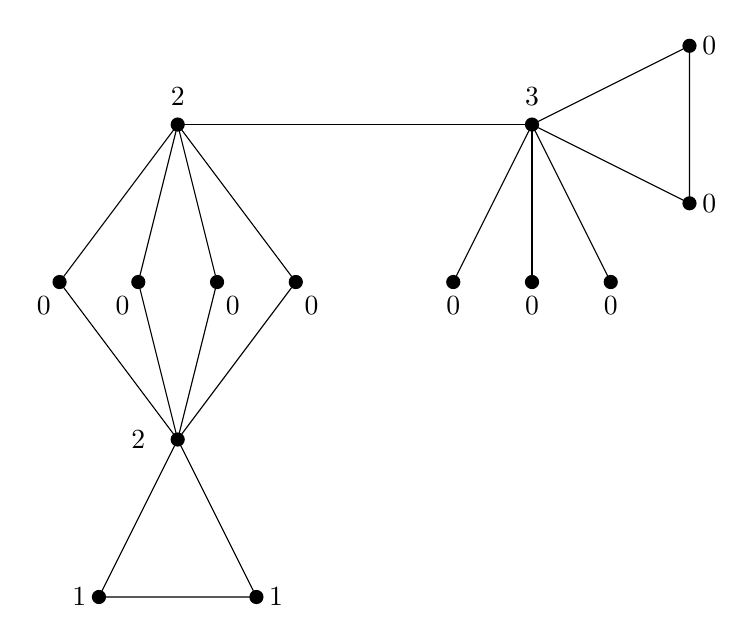
\begin{tikzpicture}
\node [draw, shape=circle,fill=black,scale=0.5] (b1) at  (2,5) {};
\node [draw, shape=circle,fill=black,scale=0.5] (b2) at  (3,5) {};
\node [draw, shape=circle,fill=black,scale=0.5] (b3) at  (4,5) {};
\node [draw, shape=circle,fill=black,scale=0.5] (b4) at  (5,5) {};
\node [draw, shape=circle,fill=black,scale=0.5] (b5) at  (7,5) {};
\node [draw, shape=circle,fill=black,scale=0.5] (b6) at  (8,5) {};
\node [draw, shape=circle,fill=black,scale=0.5] (b7) at  (9,5) {};
\node [draw, shape=circle,fill=black,scale=0.5] (b8) at  (10,6) {};
\node [draw, shape=circle,fill=black,scale=0.5] (b9) at  (10,8) {};
\node [draw, shape=circle,fill=black,scale=0.5] (a2) at  (8,7) {};
\node [draw, shape=circle,fill=black,scale=0.5] (a1) at  (3.5,7) {};
\node [draw, shape=circle,fill=black,scale=0.5] (c1) at  (3.5,3) {};
\node [draw, shape=circle,fill=black,scale=0.5] (c2) at  (2.5,1) {};
\node [draw, shape=circle,fill=black,scale=0.5] (c3) at  (4.5,1) {};

\draw(a1)--(a2);
\draw(a1)--(b1);\draw(a1)--(b2);\draw(a1)--(b3);\draw(a1)--(b4);
\draw(a2)--(b5);\draw(a2)--(b6);\draw(a2)--(b7);
\draw(a2)--(b8)--(b9)--(a2);
\draw(c1)--(b1);\draw(c1)--(b2);\draw(c1)--(b3);\draw(c1)--(b4);
\draw(c1)--(c2)--(c3)--(c1);
\node at (8,7.35)  {$3$} {};
\node at (3.5,7.35)  {$2$} {};
\node at (10.25,6)  {$0$} {};
\node at (10.25,8)  {$0$} {};
\node at (1.8,4.7)  {$0$} {};
\node at (2.8,4.7)  {$0$} {};
\node at (4.2,4.7)  {$0$} {};
\node at (5.2,4.7)  {$0$} {};
\node at (3,3)  {$2$} {};
\node at (2.25,1)  {$1$} {};
\node at (4.75,1)  {$1$} {};
\node at (7,4.7)  {$0$} {};
\node at (8,4.7)  {$0$} {};
\node at (9,4.7)  {$0$} {};


\end{tikzpicture}

\end{document}